\providecommand{\main}{..} 
\documentclass[../Master_report2.tex]{subfiles} 

\begin{document}

%\makeatletter
%\@author
%\makeatother
% full page
\begin{titlepage} %Page de garde!!
%logos de page de garde
\begin{figure}
\noindent
\begin{minipage}{0.5\textwidth}
\centering
%
\includegraphics[width=0.5\linewidth,left]{fig/leca.jpg}
\makeatletter
\@logolab
\makeatother
\end{minipage}
\begin{minipage}{0.5\textwidth}
\centering

\includegraphics[width=0.5\linewidth,right]{fig/UGA.jpg}
\end{minipage}
\end{figure}

\begin{figure}
\vskip .5em
\begin{center}
\begin{minipage}{15cm}
\centering
\noindent
\Large
\textbf{Master 2e année Biodiversité Ecologie Evolution} \\
Parcours Dynamique et modélisation de la biodiversité (DynaMo)
\normalsize
\end{minipage}
\end{center}
\end{figure}

\makeatletter
\begin{center}
~ \\
%\vskip .5em
\LARGE 
\@title 
\vskip .5em
\large
\@author \\
\@date \\
\normalsize
\end{center}
\makeatother    
    
%\maketitle
~ \vskip .5em
\hrule

\noindent
\begin{minipage}{1.8in}
\textbf{\underline{Encadrant :}} \\
\makeatletter
\@tutor
\makeatother
\end{minipage}
\hfill
\begin{minipage}{1.3in}
\textbf{\underline{Laboratoire :}} \\
\makeatletter
\@labo
\makeatother
\end{minipage}
\hfill
\begin{minipage}{1.3in}
\textbf{\underline{Équipe :}} \\
\makeatletter
\@team
\makeatother
\end{minipage}

\noindent
\begin{minipage}{1.8in}

\end{minipage}
\hfill
\begin{minipage}{3.55in}
\makeatletter
\@labadr
\makeatother
\end{minipage}

%image sympas
\begin{figure}[h]
\begin{center}
%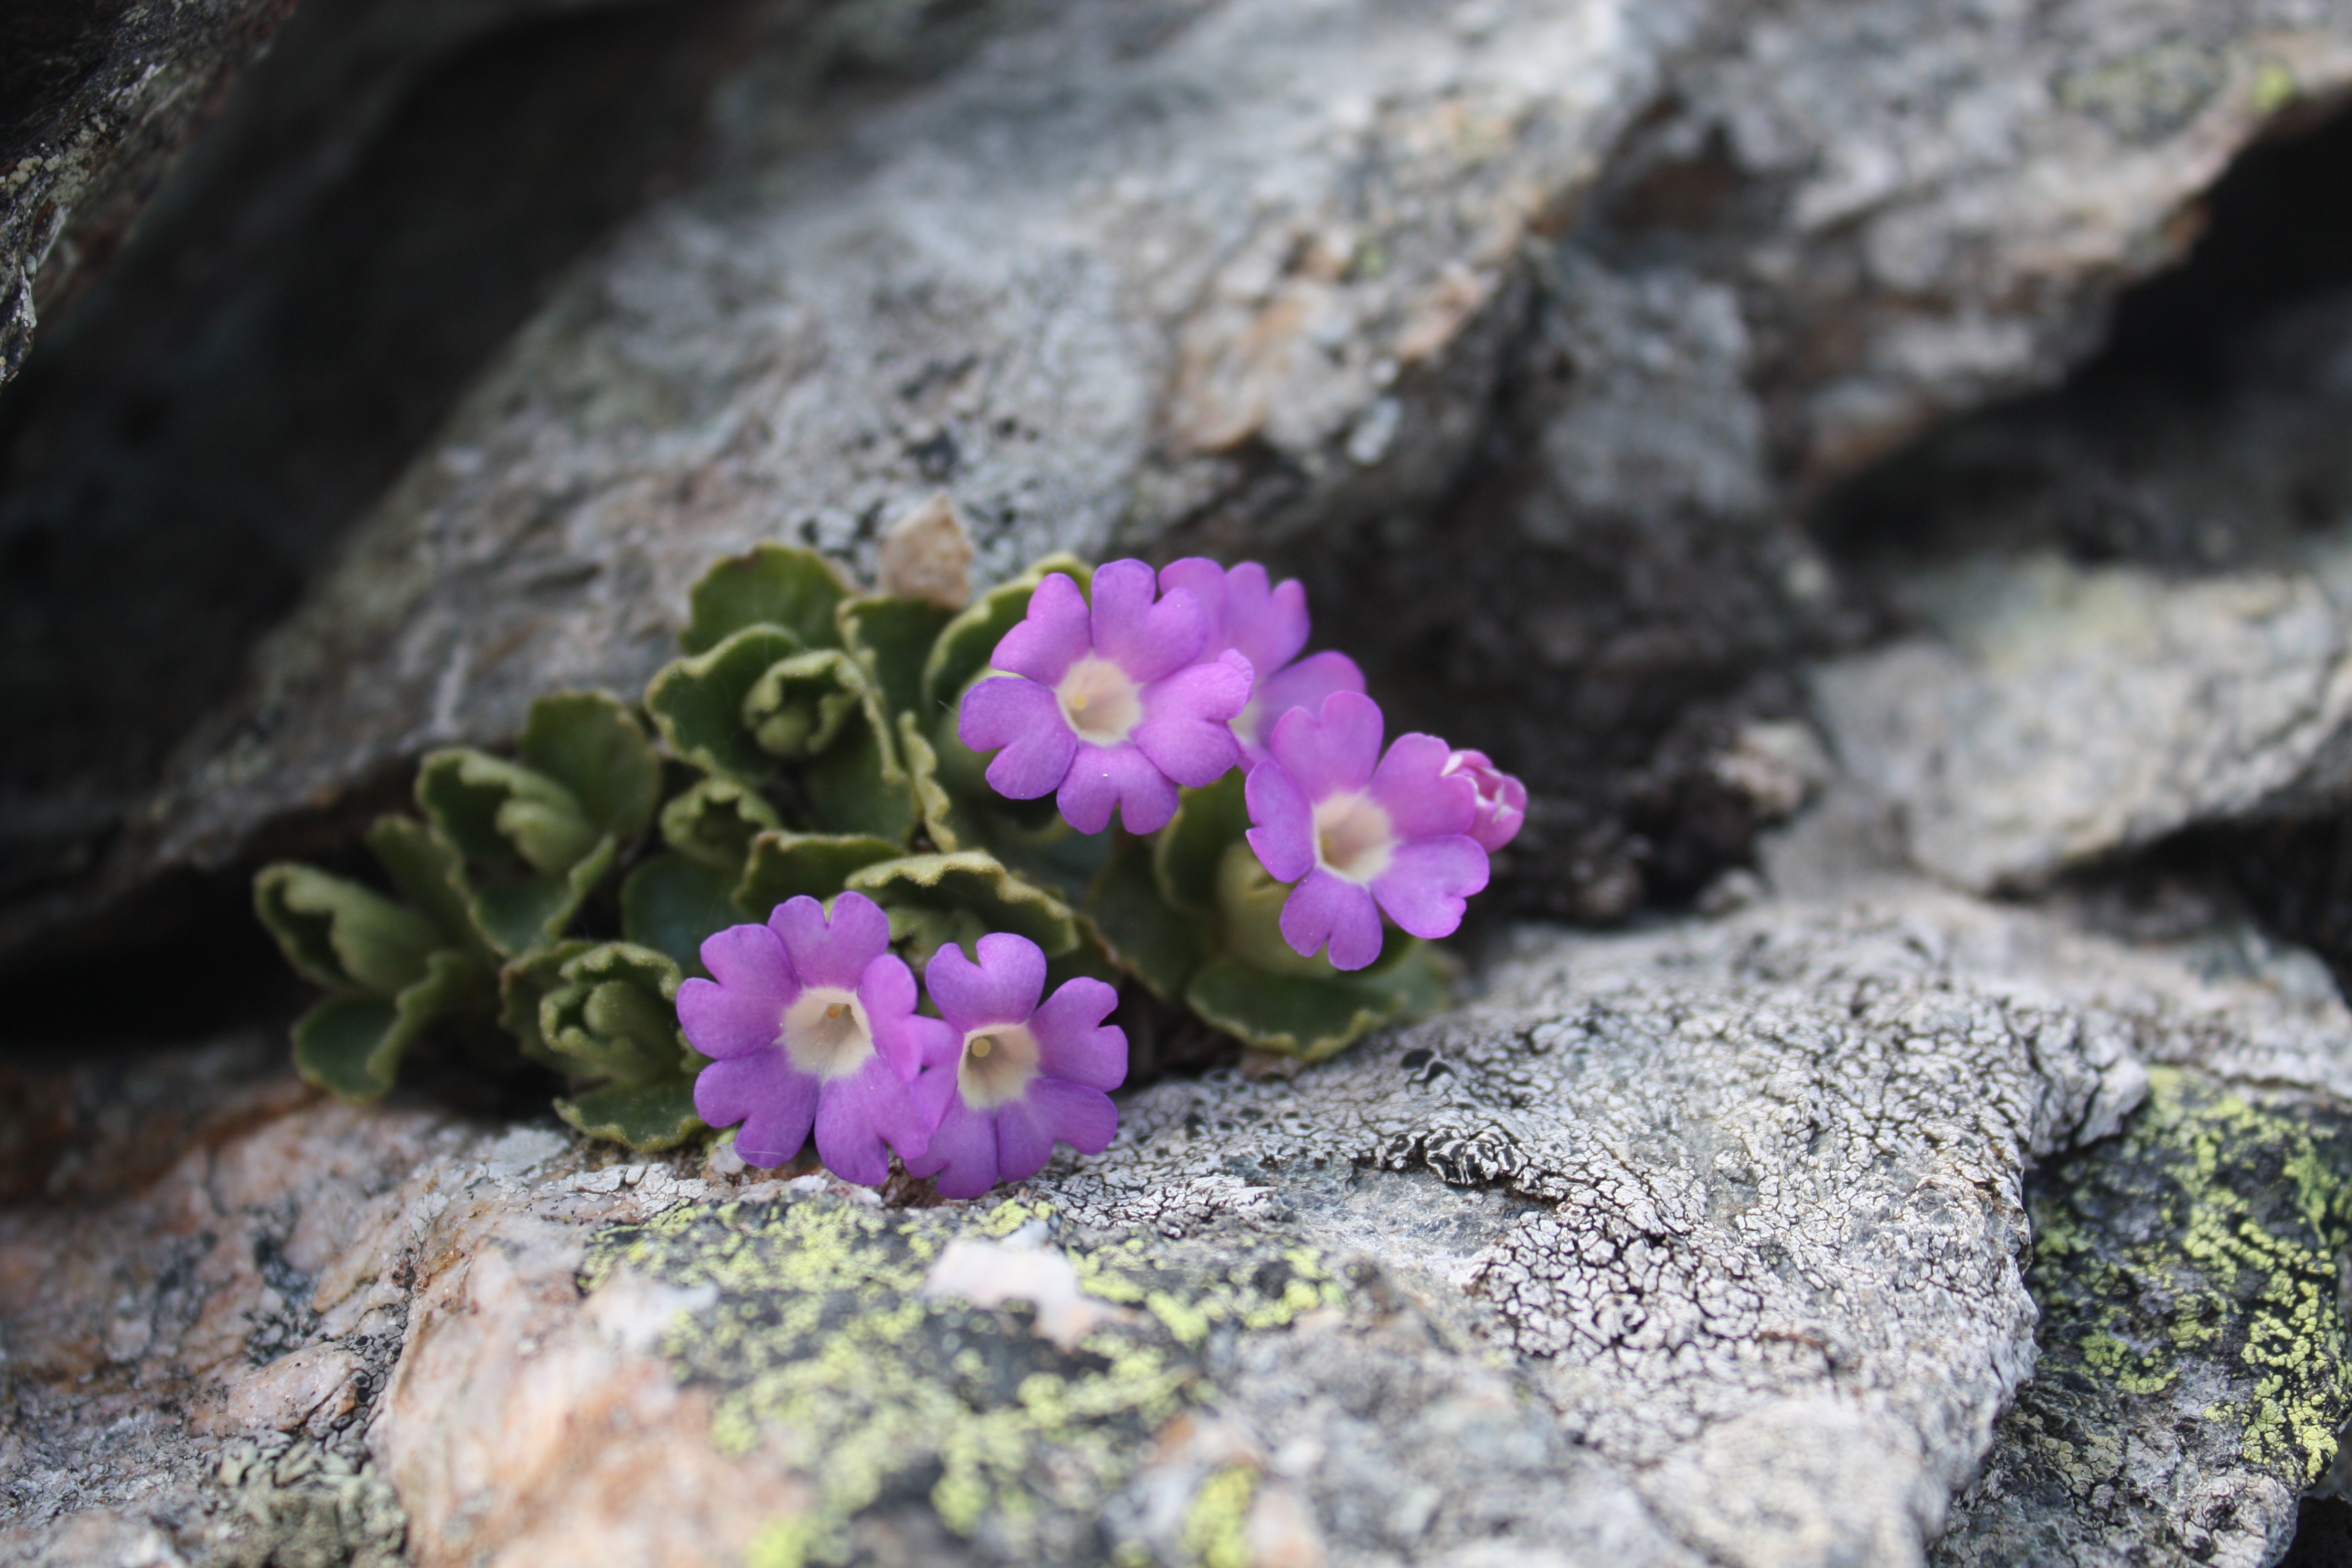
\includegraphics[height = 7cm]{fig/Primula_hirsuta_Grand_Chat_longistyle.JPG}
\makeatletter
\@pict
\makeatother
\end{center}
\end{figure}
\thispagestyle{empty}

%\makeatletter
%\@credpict
%\makeatother

\renewcommand{\footnoterule}{%
  \kern -3pt
  \hrule width \textwidth height 1pt
  \kern 2pt
}

%\makeatletter
%\@credpict
%\makeatother

\let\thefootnote\relax\makeatletter\footnote{{%\noindent 
\@credpict
~|~Contact:  \href{mailto:\@email%maxime.jaunatre@etu.univ-grenoble-alpes.fr
}{Mail $^1$}} 
\hfill \textbf{Année 2019-2020}\\
Université Grenoble Alpes - UFR de Chimie Biologie B.P.53 38041 Grenoble Cedex 9}
\makeatother


\end{titlepage}

\end{document}
